%{
%  \centering
%    \section{John Hendry Park (Trout Lake)}
%}

%\title{John Hendry Park (Trout Lake)}
%\maketitle

\begin{center}
\textsc{\LARGE Birdwatching in John Hendry Park}\\[0.2cm]
\textsc{\Large (Trout Lake)}\\[0.2cm]
\end{center}

\begin{figure}[h]
  \centering
  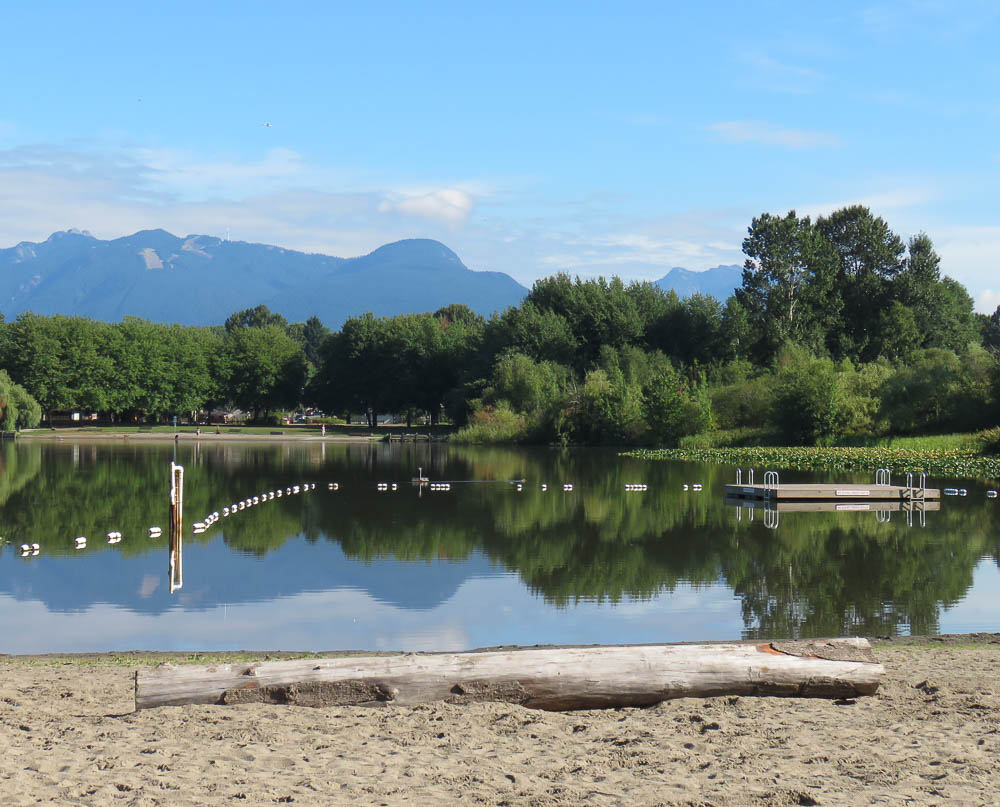
\includegraphics[width=\textwidth]{photos/TL1}
\end{figure}

\large
John Hendry Park is a 27 hectare park located in the heart of East Vancouver. 
Commonly known as Trout Lake, after the body of water in the centre of the park, the 
park itself is named after the owner of one of Vancouver's first lumber mills. 

Easily accessed from Commercial Drive, Nanaimo St, or East 12th Ave, it is a popular location 
for birders and nature-lovers alike. The park is also home to the 
Trout Lake Community Centre which provides many services to the local community. 
Over 135 bird species have been observed at Trout Lake, including seven of conservation concern.
The highest diversity of birds occurs during spring and fall migration, however
winter is also good for birdwatching as many species of waterfowl spend the season there.

